\chapter{Exploring and implementing thermodynamic models for complex liquid in open-source software PyCalphad} \label{chap:models}

\section{Introduction} \label{models:sec:intro}
For the modeling of complex liquids, Section \ref{method:ssec:liqmodels} discusses popular models within the CALPHAD framework, and Chapter \ref{chap:moltensalts} presents the applications in modeling of molten salts. Other models are also frequently applied in the chemical community to predict the nonideal mixing and phase behavior of small or large molecules. The UNIversal QUAsiChemical model (UNIQUAC) \cite{abrams1975statistical}, which considers the size and shape of ions in the solution, is currently being implemented into PyCalphad. The overall strategy for the implementation of UNIQUAC is based on three primary stages: (1) understanding and hard coding of the model, (2) representing the model through logic in code, and (3) using symbolic representation of variables used in PyCalphad as well as develop a parser for the database that use the UNIQUAC. The predicted thermochemical properties were compared with those from the OpenCalphad software \cite{li2020implementation} to verify the implementation work. Figure \ref{models:fig:implflow} shows the workflow for implementing custom models into PyCalphad and ESPEI. Moreover, a template generator is provided to expedite the process, creating templates for PyCalphad model classes and XML database schemas. These advancements provide the community with extensive opportunities to explore thermodynamic modeling with UQ in complex liquids such as molten salts, thereby making the existing databases continually updatable for the CALPHAD community and beyond. 

\begin{figure}[H]
    \centering
    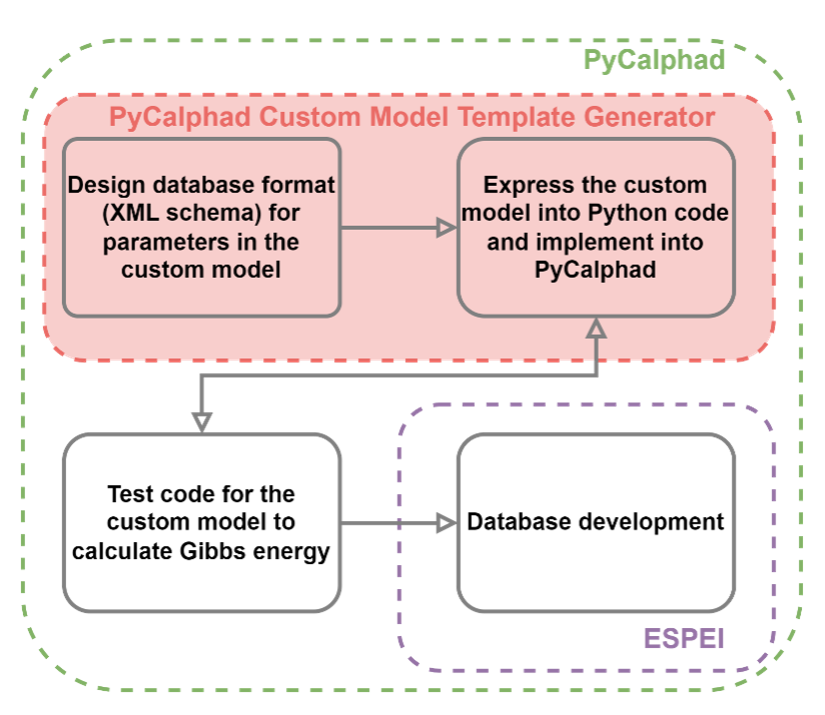
\includegraphics[width=0.75\linewidth]{models/Models-ImplementationFlow.png}
    \caption{Workflow for implementing custom models into PyCalphad and ESPEI.}
    \label{models:fig:implflow}
\end{figure}

\section{Implementation of UNIversal QUAsiChemical Model} \label{models:sec:UNIQUAC}
\subsection{UNIQUAC model} \label{models:ssec:UNIQUACfund}
The UNIQUAC model can be expressed using the CALPHAD nomenclature as follows:
\begin{equation} \label{models:eq:UQCGm}
    G_m=\sum_ix_i(^{o}G_i+RT\ln x_i) +\:^{cmb}G_m +\:^{res}G_m
\end{equation}
where $x_i$ is the mole fraction of constituent $i$, ${^o}G_i$ is the reference Gibbs energy of $i$, $\sum_ix_i^{o}G_i$ is considered as $^{srf}G_m$ term in (\ref{method:eq:Gm}). The second term $RT\sum_ix_i\ln x_i$ is configurational entropy contribution to Gibbs energy as $-T\:^{cnf}S_m$ term in (\ref{method:eq:Gm}). The excess Gibbs energy $^{xs}G_m$ are considered into two parts in the UNIQUAC, i.e., $^{cmb}G_m$ the combinatorial contribution of Gibbs energy and $^{res}G_m$ is the residual contribution of Gibbs energy.  

$^{cmb}G_m$ can be expressed as:
\begin{equation} \label{models:eq:UQCGcmb}
    ^{cmb}G_m=RT\sum_{i}{x_i\ln(\frac{\mathrm{\Phi}_i}{x_i}})+\frac{z}{2}\sum_{i}{x_iq_i\ln(\frac{\theta_i}{\mathrm{\Phi}_i}})
\end{equation}
\begin{equation} \label{models:eq:UQCphi}
    \mathrm{\Phi}_i=\frac{r_{i}x_i}{\sum_{j}{{r}_{j}x_j}}
\end{equation}
\begin{equation} \label{models:eq:UQCtheta}
    \theta_i= \frac{q_{i}x_i}{\sum_{j}{{q}_{j}x_j}}
\end{equation}
where $x_i$ is the mole fraction of constituent $i$, $r_i$ and $q_i$ are the component structural parameters, $r_i$ is the volume parameter, $q_i$ is the surface-area parameter, and $z$ is the average number of the nearest neighbors. $^{res}G_m$ can be expressed as:
\begin{equation} \label{models:eq:UQCres}
    {^{res}}G_m=-RT\sum_{i}{x_iq_i\ln(\rho_i})
\end{equation}
\begin{equation} \label{models:eq:rho}
    \rho_i=\sum_{j}{\theta_j\tau_{ji}}
\end{equation}
\begin{equation} \label{models:eq:UQCtau}
    \tau_{ji}=\exp \left(-\frac{u_{ij}-u_{ii}}{RT}\right)
\end{equation}
where $\Delta u_{ij}=u_{ij}-u_{ii}$ is the interaction parameter between $i$ and $j$, $u_{ii}$ represents the property of pure $i$. Thus, $\Delta u_{ij} \neq \Delta u_{ji}$ and $\tau_{ji} \neq \tau_{ij}$ Usually, $\Delta u_{ij}$ can be treated together as adjustable parameters during the modeling process.

%%%XML Database
To implement UNIQUAC into PyCalphad, a thermodynamic database containing the necessary parameters, such as $r_i$, $q_i$, and $\Delta u_{ij}$, is required. This database allows users to define these parameters, which PyCalphad can then read. To manage these newly defined parameters, an XML schema is employed as follows:
\begin{minted}[xleftmargin=1\parindent, linenos=true, fontsize=\small, breaklines=true]{xml}
<element name="Parameter">
    <attribute name="type">
        <choice>
            <value>UQCG</value><a:documentation>Gibbs energy of a specie</a:documentation>
            <value>UQCT</value><a:documentation>Tau function in residual contribution of excess Gibbs energy</a:documentation>
            <value>UQCQ</value><a:documentation>Surface-area parameter</a:documentation>
            <value>UQCR</value><a:documentation>Volume parameter</a:documentation>
            <value>UQCZ</value><a:documentation>Coordination number of a constituent</a:documentation>
        </choice>
    </attribute>
    <interleave>
        <optional>
            <text/>
        </optional>
        <zeroOrMore>
            <ref name="Interval"/>
        </zeroOrMore>
        <ref name="UNIQUACConstituentArray"/>
        <optional>
            <element name="Exponents">
                <list>
                    <data type="float"/>
                    <data type="float"/>
                </list>
            </element>
        </optional>
    </interleave>
</element>
\end{minted}
Here are the parts of the XML schema where parameters are defined. For example, by specifying \texttt{UQCQ}, the surface-area parameter $q_i$ can be defined. \texttt{UQCG} is the reference Gibbs energy ${^o}G_i$ in the (\ref{models:eq:UQCGm}), \texttt{UQCT} is the $\tau_{ji}$ function in residual contribution of excess Gibbs energy as shown in (\ref{models:eq:UQCtau}), \texttt{UQCR} is the volume parameter $r_i$, and \texttt{UQCZ} is the coordination number $z$.

The users now can adopt an XML thermodynamic database to input these parameters.
\begin{minted}[xleftmargin=1\parindent, linenos=true, fontsize=\small, breaklines=true]{xml}
<Parameter type='UQCQ'>1.72<ConstituentArray><Site refid="0"><Constituent refid="ACETONITRILE"/></Site></ConstituentArray></Parameter>
<Parameter type='UQCR'>1.87<ConstituentArray><Site refid="0"><Constituent refid="ACETONITRILE"/></Site></ConstituentArray></Parameter>
<Parameter type='UQCQ'>4.4<ConstituentArray><Site refid="0"><Constituent refid="N_HEPTANE"/></Site></ConstituentArray></Parameter>
<Parameter type='UQCR'>5.17<ConstituentArray><Site refid="0"><Constituent refid="N_HEPTANE"/></Site></ConstituentArray></Parameter>
<Parameter type="UQCZ">10<ConstituentArray><Site refid="0"><Constituent refid="ACETONITRILE"/></Site></ConstituentArray></Parameter>
<Parameter type="UQCZ">10<ConstituentArray><Site refid="0"><Constituent refid="N_HEPTANE"/></Site></ConstituentArray></Parameter>
<Parameter type="UQCT">exp(VV0001*T**(-1))<ConstituentArray><Site refid="0"><Constituent refid="ACETONITRILE"/><Constituent refid="N_HEPTANE"/></Site></ConstituentArray><Exponents>0.0 1.0</Exponents></Parameter>
<Parameter type="UQCT">exp(-545.71*T**(-1))<ConstituentArray><Site refid="0"><Constituent refid="ACETONITRILE"/><Constituent refid="N_HEPTANE"/></Site></ConstituentArray><Exponents>1.0 0.0</Exponents></Parameter>
\end{minted}

Here is an example of how to specify parameters for UNIQUAC in an XML thermodynamic database. First, define the type of parameter, such as \texttt{UQCQ}. Then, specify the value or function for that parameter. Following this, the name of the constituent can be defined using the \texttt{Constituent} tag.

\subsection{Calculations examples} \label{models:ssec:UNIQUACexamples}
With the implementation of the new UNIQUAC model in PyCalphad, users can automatically utilize all existing features in PyCalphad, including Gibbs energy minimization and phase diagram plotting. First, the calculation of Gibbs energy and its derivatives are carried out as a benchmark, comparing with calculation results from OpenCalphad \cite{li2020implementation}.

Figure \ref{models:fig:UQCGibbsE}, Figure \ref{models:fig:UQCS}, and Figure \ref{models:fig:UQCacr} depict the comparison between PyCalphad and OpenCalphad for calculating Gibbs energy, entropy, and activity, respectively. In PyCalphad, the \textit{calculate()} function was used to sample properties of a single phase, while the \textit{equilibrium()} function was utilized to perform global minimization of Gibbs energies and obtain phase equilibria. Both functions were thoroughly tested for UNIQUAC to ensure accurate calculations and minimization of Gibbs energy. The results demonstrate an excellent agreement between PyCalphad and OpenCalphad. The detailed value of Gibbs energy, entropy, and activity calculations are listed in Table \ref{models:tab:UQCGibbsE}, Table \ref{models:tab:UQCS}, and Table \ref{models:tab:UQCacr}, which shows that 0\% difference between calculations by PyCalphad and OpenCalphad. These calculations affirm the successful implementation of UNIQUAC in PyCalphad.

\begin{figure}[H]
    \centering
    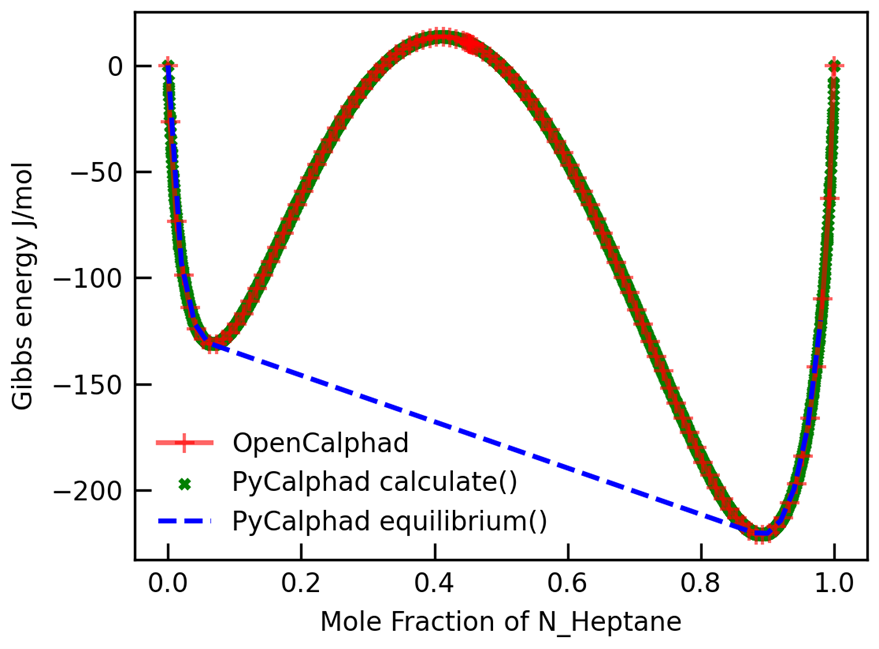
\includegraphics[width=0.5\linewidth]{models/Models-UQC-Gibbsenergy.png}
    \caption{Comparison of PyCalphad with OpenCalphad calculating Gibbs energy to verify the implementation of UNIQUAC. The red line represents results from OpenCalphad, the green $\times$ symbols represent results from the PyCalphad \textit{calculate()} function, and the blue line represents results from the PyCalphad \textit{equilibrium()} function.}
    \label{models:fig:UQCGibbsE}
\end{figure}

\begin{table}[H]
    \centering
    \caption{The Gibbs energy value calculated from PyCalphad compared to values from OpenCalphad at four different compositions.}
    \begin{tabular}{>{\raggedright\arraybackslash}m{1.5cm}>{\raggedright\arraybackslash}m{3.5cm}>{\raggedright\arraybackslash}m{3.5cm}>{\raggedright\arraybackslash}m{3.5cm}}
    \hline
         \textbf{$x_i$}&\textbf{PyCalpahd}&\textbf{OpenCalphad}&\textbf{Relative difference}\\
    \hline
        0.05&$-127.817$&$-127.817$&0\%\\
        0.1&$-135.093$&$-135.093$&0\%\\
        0.5&$-178.744$&$-178.744$&0\%\\
        0.9&$-220.393$&$-220.393$&0\%\\
    \hline
    \end{tabular}
    \label{models:tab:UQCGibbsE}
\end{table}

\begin{figure}[H]
    \centering
    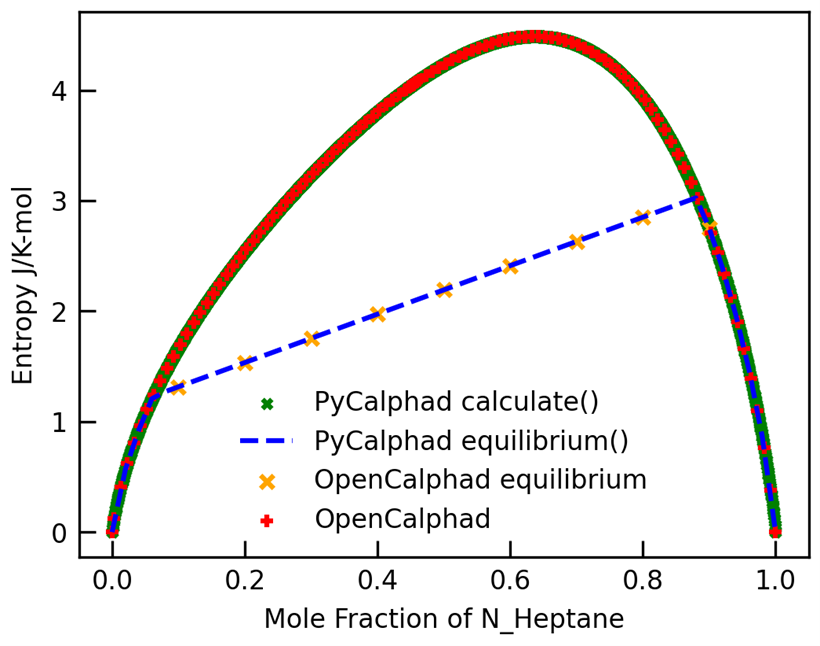
\includegraphics[width=0.5\linewidth]{models/Models-UQC-Entropy.png}
    \caption{Comparison of PyCalphad with OpenCalphad calculating entropy to verify the implementation of UNIQUAC. The red line represents results from OpenCalphad, the yellow $\times$ symbols represent results from OpenCalphad equilibrium calculations, the green $\times$ symbols represent results from the PyCalphad \textit{calculate()} function, and the blue line represents results from the PyCalphad \textit{equilibrium()} function.}
    \label{models:fig:UQCS}
\end{figure}

\begin{table}[H]
    \centering
    \caption{The entropy value calculated from PyCalphad compared to values from OpenCalphad at four different compositions.}
    \begin{tabular}{>{\raggedright\arraybackslash}m{1.5cm}>{\raggedright\arraybackslash}m{3.5cm}>{\raggedright\arraybackslash}m{3.5cm}>{\raggedright\arraybackslash}m{3.5cm}}
    \hline
         \textbf{$x_i$}&\textbf{PyCalpahd}&\textbf{OpenCalphad}&\textbf{Relative difference}\\
    \hline
        0.1&1.315&1.315&0\%\\
        0.3&1.754&1.754&0\%\\
        0.5&2.192&2.192&0\%\\
        0.9&2.752&2.752&0\%\\
    \hline
    \end{tabular}
    \label{models:tab:UQCS}
\end{table}

\begin{table}[H]
    \centering
    \caption{The activity value calculated from PyCalphad compared to values from OpenCalphad at four different compositions.}
    \begin{tabular}{>{\raggedright\arraybackslash}m{1.5cm}>{\raggedright\arraybackslash}m{3.5cm}>{\raggedright\arraybackslash}m{3.5cm}>{\raggedright\arraybackslash}m{3.5cm}}
    \hline
         \textbf{$x_i$}&\textbf{PyCalpahd}&\textbf{OpenCalphad}&\textbf{Relative difference}\\
    \hline
        0.05&0.11376&0.11376&0\%\\
        0.3&0.28710&0.28710&0\%\\
        0.5&0.47857&0.47857&0\%\\
        0.9&0.89851&0.89851&0\%\\
    \hline
    \end{tabular}
    \label{models:tab:UQCacr}
\end{table}

\begin{figure}[H]
    \centering
    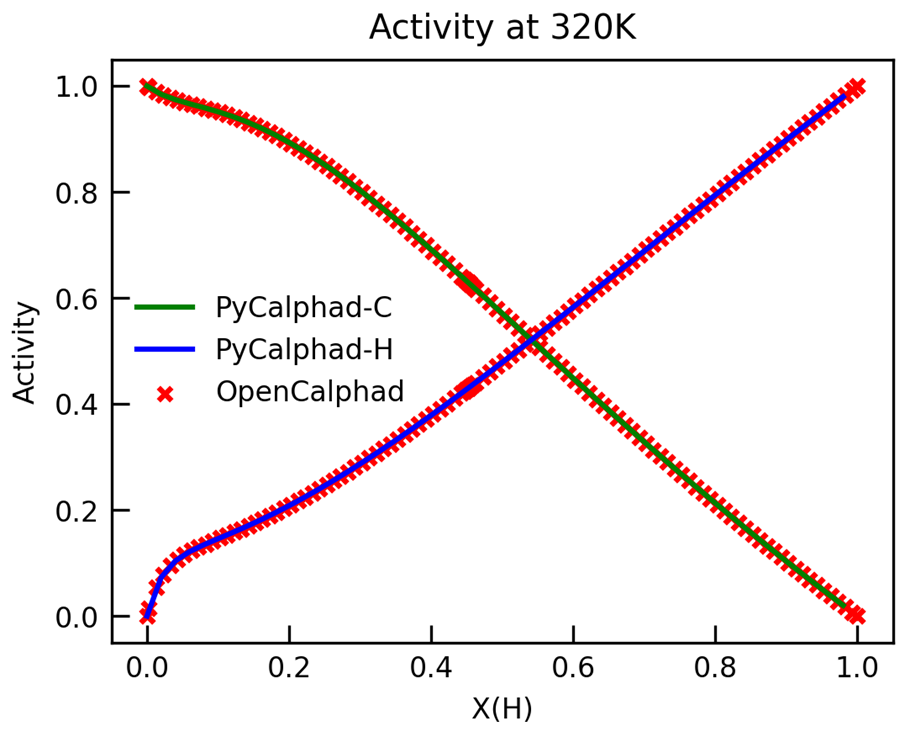
\includegraphics[width=0.5\linewidth]{models/Models-UQC-Activity.png}
    \caption{Comparison of PyCalphad with OpenCalphad calculating activity to verify the implementation of UNIQUAC. The red $\times$ symbols represent results from OpenCalphad; green and blue lines are calculated from PyCalphad.}
    \label{models:fig:UQCacr}
\end{figure}

\begin{figure}[H]
    \centering
    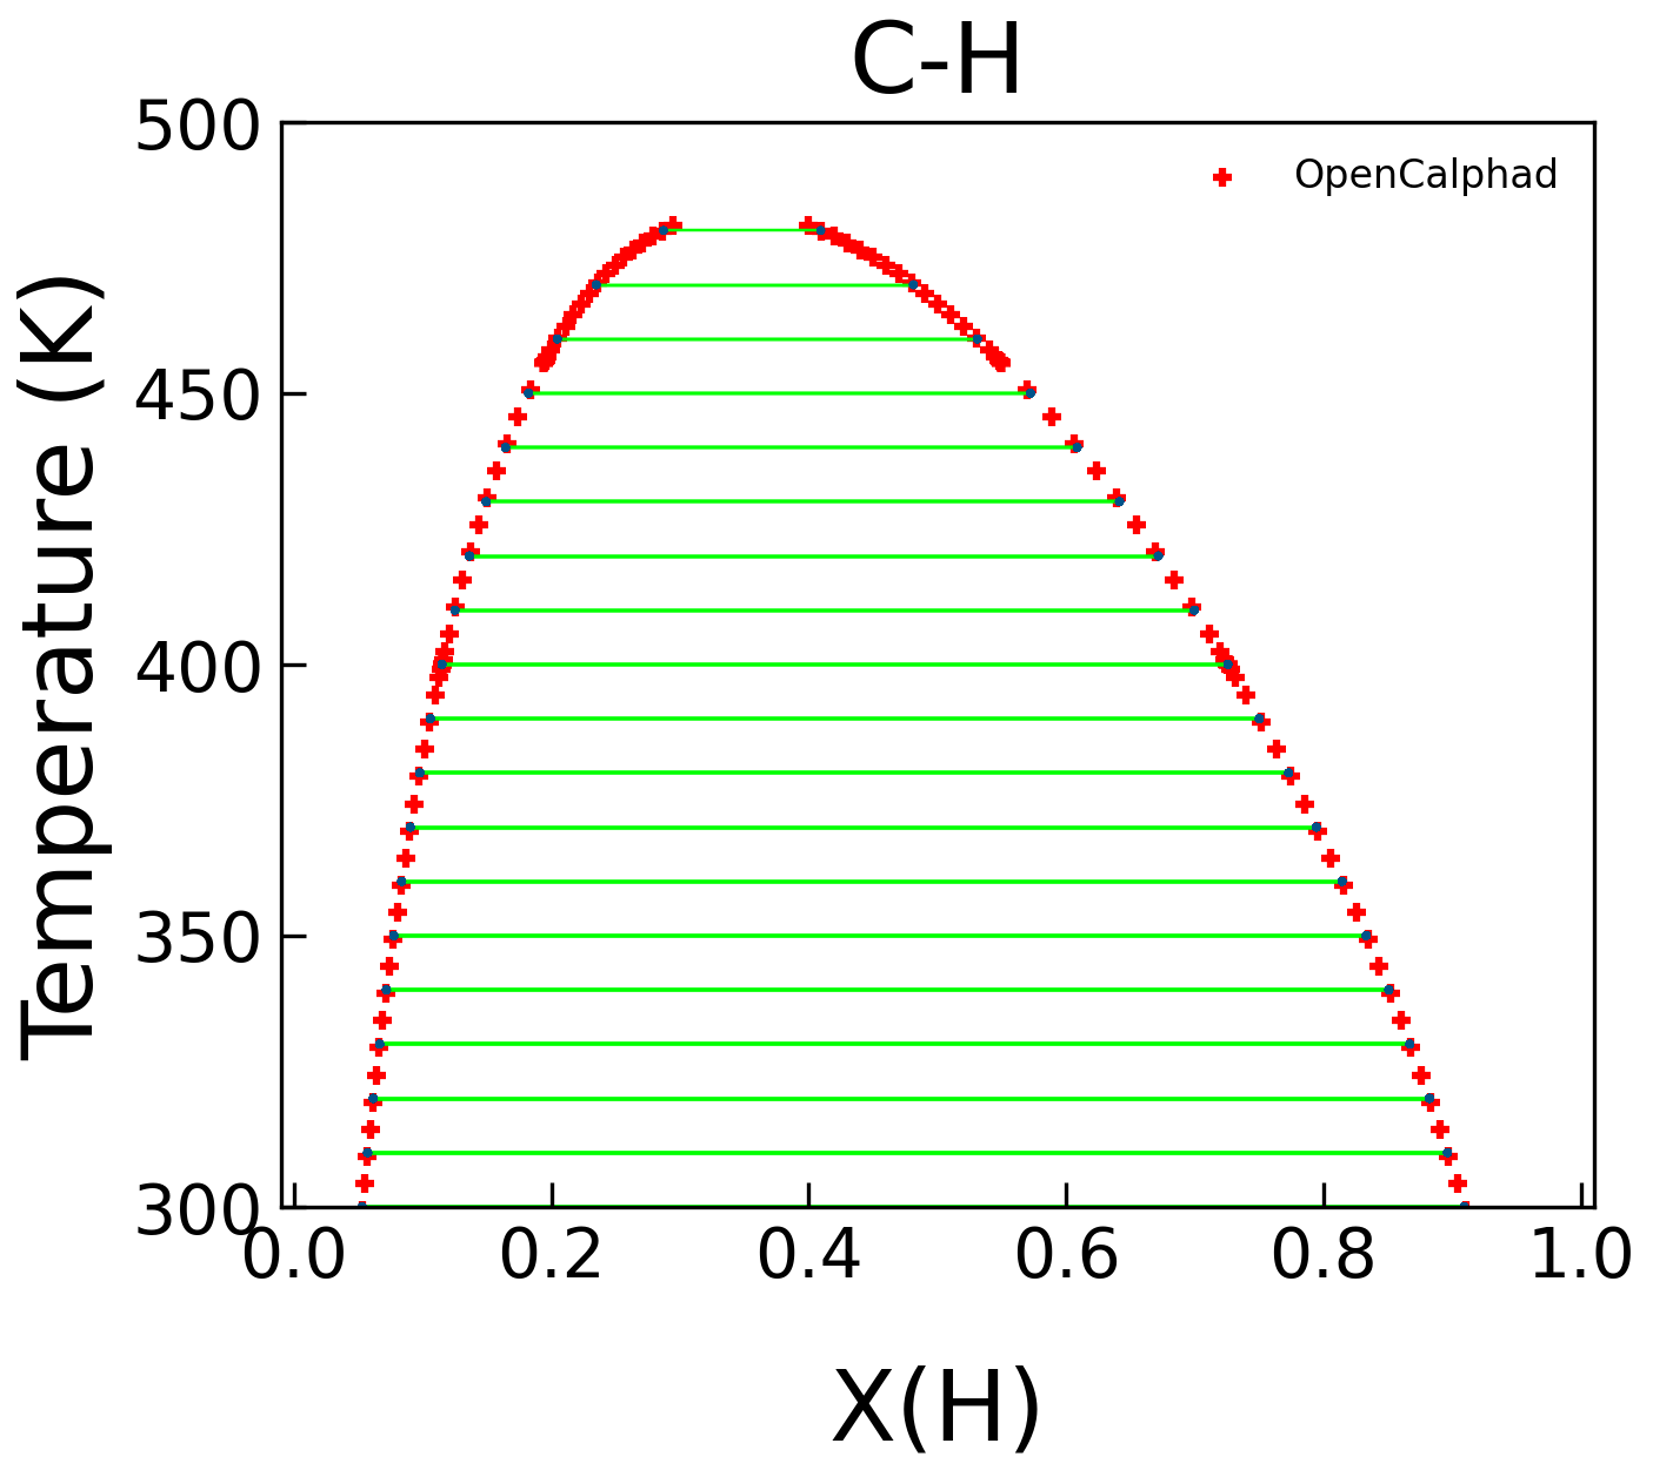
\includegraphics[width=0.5\linewidth]{models/Models-UQC-BinaryPD.png}
    \caption{Comparison of PyCalphad with OpenCalphad calculating the binary phase diagram to verify the implementation of UNIQUAC. The red $+$ symbols represent results from OpenCalphad; green lines are tie lines calculated from PyCalphad.}
    \label{models:fig:UQCBinary}
\end{figure}

\begin{figure}[H]
    \centering
    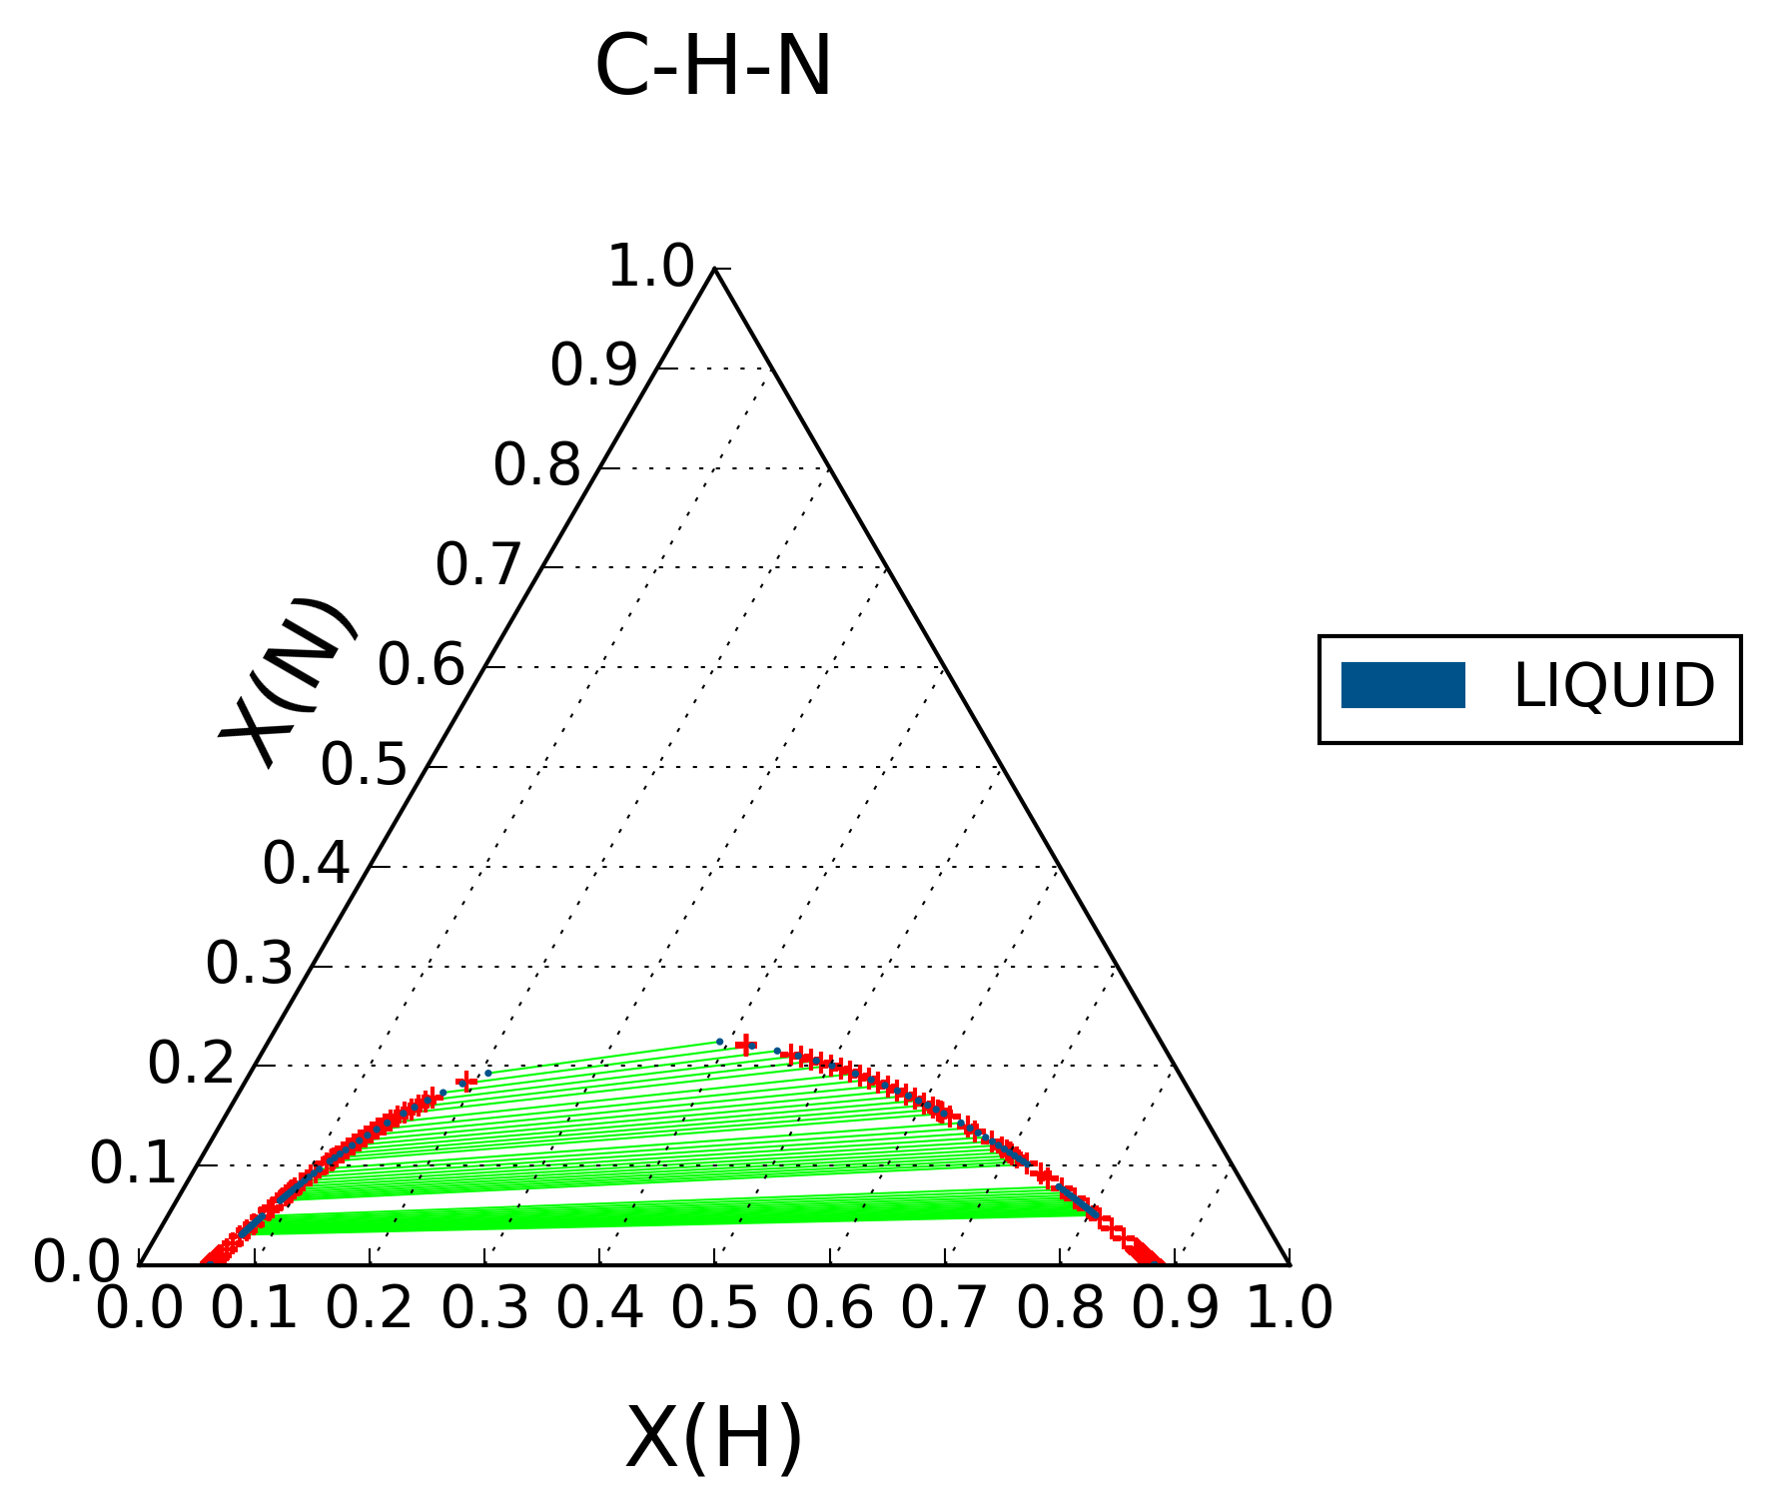
\includegraphics[width=0.5\linewidth]{models/Models-UQC-TernaryPD.png}
    \caption{Comparison of PyCalphad with OpenCalphad calculating the ternary phase diagram to verify the implementation of UNIQUAC. The red $+$ symbols represent results from OpenCalphad; green lines are tie lines calculated from PyCalphad.}
    \label{models:fig:UQCTernary}
\end{figure}

Figure \ref{models:fig:UQCBinary} and Figure \ref{models:fig:UQCTernary} shows the binary and ternary phase diagram for an artificial system modeled with UNIQUAC calculated from PyCalphad. The phase boundary matches well with phase diagram data obtained using OpenCalphad. These calculations and plots were generated using the existing functions in PyCalphad, namely \textit{equilibrium()} and \textit{eqplot()}. This alignment underscores the success of the UNIQUAC implementation in PyCalphad and demonstrates the robustness and capability of PyCalphad's existing functions for custom thermodynamic models.

\section{Custom model template generator} \label{models:sec:CMTG}
\subsection{Framework} \label{models:ssec:CMTGframework}
As illustrated in Figure \ref{models:fig:implflow}, implementing any custom model in PyCalphad requires an XML schema for the thermodynamic database and a corresponding class for PyCalphad model codes. To enhance the efficiency of adding new models and to minimize conflicts arising from format styles in PyCalphad, a custom model template generator has been developed. Figure \ref{models:fig:CMGFrame} shows the framework of this custom model template generator.

\begin{figure}[H]
    \centering
    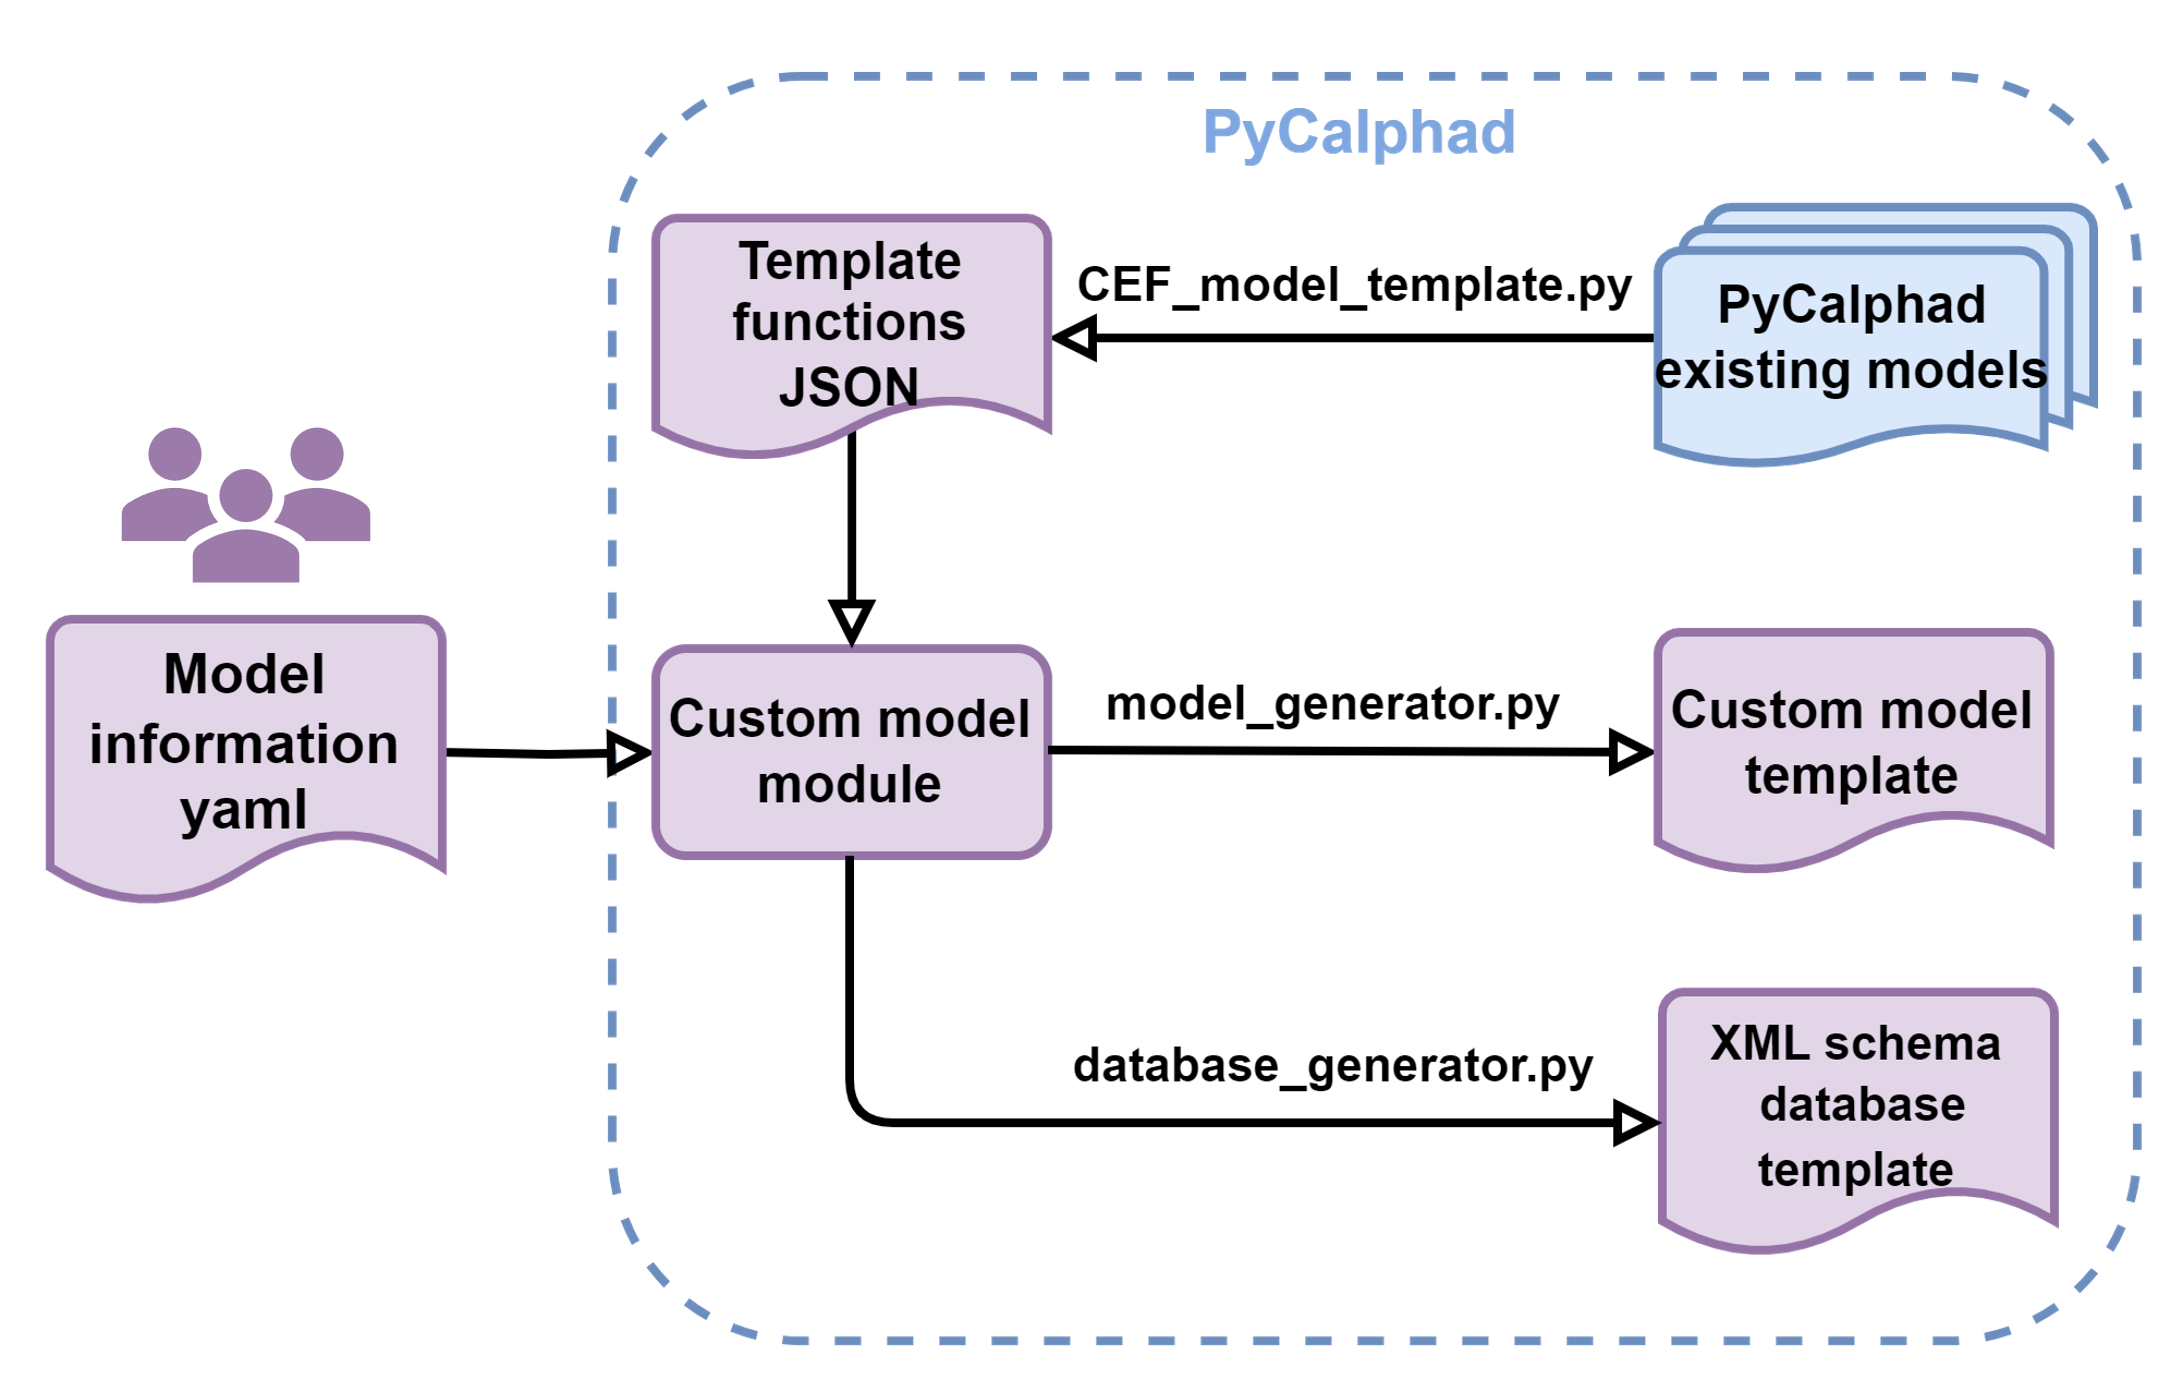
\includegraphics[width=0.8\linewidth]{models/Models-CMG-Framework.png}
    \caption{The framework of the custom model template generator.}
    \label{models:fig:CMGFrame}
\end{figure}

To use this template generator, a configuration YAML file is required to input model information, including model name, model parameters, etc. Below is an example of keywords in the model information YAML file:
\begin{minted}[xleftmargin=1\parindent, linenos=true, fontsize=\small, breaklines=true]{yaml}
    model:
      name
      energy_contributions
      basic_functions
      parameters_functions
        - parameter
          attributes
          database_keyword
          comments
      energy_functions
        - energy
          function
          comments

    database:
      name
      description
      parameters
      options
\end{minted}
There are two sections in this YAML file. The \texttt{model} key is intended to define the custom model and generate a template Python code for a PyCalphad model class. The \texttt{name} key is for input the name of the custom model. The \texttt{energy$\_$contribution}s keyword is to define what contributions to Gibbs energy are considered in the custom model. For example, in CEF, four contributions, $^{srf}G_m$, $^{cnf}S_m$, $^{xs}G_m$, and $^{phys}G_m$ are considered, while in UNIQUAC, $^{srf}G_m$, $^{cnf}S_m$, $^{cmb}G_m$, and $^{res}G_m$ are included. The \texttt{basic$\_$functions} defines some functions that can be extracted from existing models in PyCalphad to use in the custom model. The \texttt{parameters$\_$functions} is intended to define the functions for new parameters in the custom model. Information including parameter names, attributes, corresponding keywords defined in the database, and other comments for the parameter can be provided within this keyword. The \texttt{energy$\_$functions} is for the functions for energy contributions in the custom model, users are allowed to provide information including function name, function expression, and other comments for each energy contribution. The second section in the YAML file begins with the \texttt{database} key. This key is intended to define the XML database schema and generate a template XML rng file for PyCalphad-xml as shown in Section \ref{models:ssec:UNIQUACfund}. The name of the custom model can be defined with the \texttt{name} key. Comments or descriptions about the custom model, such as the full name of the model, can be input with \texttt{description}. The key \texttt{parameters} is for defining the name of new parameters in the custom model. It is corresponding with the \texttt{database$\_$keyword} value under \texttt{model: parameters$\_$functions} key. The \texttt{options} key is intended to define some optional schema for parameter structures. Options include \texttt{Exponent} and \texttt{Order}.

The major two functions in the custom model template generator are \textit{model$\_$generator()} and \textit{database$\_$generator()} as shown in Figure \ref{models:fig:CMGFrame}. In addition, there is \textit{CEF$\_$model$\_$template()} function to extract functions from existing PyCalphad models and save them into \texttt{template$\_$functions.json}. Below is the usage of these functions:
\begin{minted}[xleftmargin=1\parindent, linenos=true, fontsize=\small, breaklines=true]{python}
    configuration_file='configuration_file_name'
    output_rng_file='rng_file_name.rng'
    output_model_file='model_file_name.py'
    database_generator(configuration_file, output_rng_file)
    model_generator(configuration_file, output_model_file, print_model=True)
\end{minted}
The output of using the custom model template generator includes a \texttt{rng$\_$file$\_$name.rng} and a \texttt{model$\_$file$\_$name.py}, which users can start with for further improvement and implementation into PyCalphad.

\subsection{Application: the Peng-Robinson Euqation of State} \label{models:ssec:CMTGapp} %Add PR EOS introduction and impact
The custom model template generator has been utilized to implement the Peng-Robinson equation of state (PR EOS) \cite{peng1976new}. Developed by Peng and Robinson, this model is designed to predict the behavior of substances in gas, liquid, and supercritical fluid states \cite{peng1976new}. With more than 40 years of development, there are more than 220 modifications to the PR EOS for compounds and mixtures \cite{LopezEcheverry201739}. PR EOS is highly regarded in industrial applications, particularly in the oil, gas, and petrochemical, for its effectiveness in investigating phase equilibrium. However, there is a need to enhance the optimization process for this model, where it could greatly benefit from the capabilities offered by PyCalphad and ESPEI.

The Gibbs energy derived from PR EOS can be expressed as \cite{tang2005supercritical}:
\begin{equation} \label{models:eq:PRGm}
    G_m=\sum_i{x_i\left[^{o}G_i(T, P_0)+RT\left(\ln{x_i}+\ln{\frac{\phi_iP}{P_0}}\right)\right]}
\end{equation}
where $^{o}G_i(T, P_0)$ is the reference Gibbs energy of species $i$ at temperature T and standard state pressure $P_0$, $\phi_i$ is the fugacity coefficient of species $i$, which can be expressed as:
\begin{equation} \label{models:eq:PRphi}
    \ln{\phi_i}=\frac{b_i}{b_m}(Z-1)-\ln{(Z-B^*)}-\frac{A^*}{2B^*\sqrt{2}}\left(\frac{2\sum_jx_ja_{ij}}{a_m}-\frac{b_i}{b_m}\right)\ln{\left(\frac{Z+(1+\sqrt{2}B^*)}{Z+(1-\sqrt{2}B^*)}\right)}
\end{equation}
\begin{equation} \label{models:eq:PRaij}
    a_{ij}=(a_ia_j)^{0.5}(1-k_{ij})
\end{equation}
\begin{equation} \label{models:eq:PRam}
    a_m=\sum_i\sum_jx_ix_ja_{ij}
\end{equation} 
\begin{equation} \label{models:eq:PRAs}
    A^*=\frac{a_m(T)P}{R^2T^2}
\end{equation}
\begin{equation} \label{models:eq:PRbm}
    b_m=\sum_ix_ib_i
\end{equation} 
\begin{equation} \label{models:eq:PRBs}
    B^*=\frac{b_mP}{RT}
\end{equation}
where $a_i$ is the Peng–Robinson temperature-dependent attraction parameter of species $i$, $k_{ij}$ is binary interaction coefficient between species $i$ and $j$, $b_i$ is the Peng–Robinson temperature-independent repulsion parameter of species $i$, $a_m$ is the mixture of $a_i$ over all species, $b_m$ is the mixture of $b_i$ over all species $i$, $A^*$ is the dimensionless form of $a_m$ for a mixture, and $B^*$ is the dimensionless form of $b_m$ for a mixture. $Z$ is the compressibility factor, which can be solved by:
\begin{equation} \label{models:eq:PRZ}
    Z^3-(1-B^*)Z^2+(A^*-2B^*-3B^{*2})Z-(A^*B^*-B^{*2}-B^{*3})=0
\end{equation}

To use the PR EOS, users need to define the parameters $a_i$, $b_i$, and $k_{ij}$ in the thermodynamic database. Additionally, the parameter functions for calculating $a_{ij}$, $a_m$, $b_m$, $A^*$, $B^*$, and $Z$ are required to be defined in the model class of PR EOS. Thus, the configuration YAML file for the PR EOS can be prepared as:
\begin{minted}[xleftmargin=1\parindent, linenos=true, fontsize=\small, breaklines=true]{yaml}
model:
  name: PRModel
  energy_contributions:
    ref: reference_energy
    idmix: ideal_mixing_energy
    xsmix: excess_mixing_energy
  basic_functions: ['default']
  parameters_functions:
    - parameter: a_i
      attributes: 
        - "i: v.Species"
      database_keyword: PRMA
      comments: Peng-Robinson temperature-dependent attraction term
    - parameter: b_i
      attributes: 
        - "i: v.Species"
      database_keyword: PRMB
      comments: Peng-Robinson temperature-independent repulsion term
    - parameter: a_ij
      attributes:
        - "i: v.Species"
        - "j: v.Species"
      database_keyword: null
      comments: (a_i*a_j)^0.5(1-k_ij)
    - parameter: a_m
      attributes: null
      database_keyword: null
      comments: sum(x_i*x_j*a_ij)
    - parameter: b_m
      attributes: null
      database_keyword: null
      comments: sum(x_i*b_i)
    - parameter: A_s
      attributes: null
      database_keyword: null
      comments: (a_m*P)/(R^2*T^2)
    - parameter: B_s
      attributes: null
      database_keyword: null
      comments: (b_m*P)/(R*T)
    - parameter: Z
      attributes: null
      database_keyword: null
      comments: solve from A_s and B_s
  energy_functions:
    - energy: reference_energy
      function: CEF-default
      comments: null
    - energy: ideal_mixing_energy
      function: CEF-default
      comments: null
    - energy: excess_mixing_energy
      function: null
      comments: fugacity

database:
  name: PRModel
  description: Peng-Robinson model
  parameters:
    PRMA: Peng-Robinson temperature-dependent attraction term
    PRMB: Peng-Robinson temperature-independent repulsion term
    PRMK: Peng-Robinson interaction parameter
  options:
   - Exponents
\end{minted}
The XML rng file for PR EOS can be obtained by running the template generator functions:
\begin{minted}[xleftmargin=1\parindent, linenos=true, fontsize=\small, breaklines=true]{python}
    configuration_file='PR_Model.yaml'
    output_file='PR_schema.rng'
    database_generator(configuration_file, output_file)
\end{minted}
The partial output of the XML rng file is shown as follows:
\begin{minted}[xleftmargin=1\parindent, linenos=true, fontsize=\small, breaklines=true]{xml}
<?xml version='1.0' encoding='utf-8'?>
...
    <include href="core.rng"/>
    <define name="PRModelConstituentArray">
        <element name="ConstituentArray">
           ...
        </element>
    </define>
    <define name="PRModel.model" combine="choice">
        <element name="Model">
            <attribute name="type">
                <a:documentation>Peng-Robinson model</a:documentation>
                <value>PRModel</value>
            </attribute>
            <interleave>
                <ref name="PRModelConstituentArray"/>
                ...
            </interleave>
        </element>
        <zeroOrMore>
            <element name="Parameter">
                <attribute name="type">
                    <choice>
                        <value>PRMA</value>
                        <a:documentation>Peng-Robinson temperature-dependent attraction term</a:documentation>
                        <value>PRMB</value>
                        <a:documentation>Peng-Robinson temperature-dependent repulson term</a:documentation>
                        <value>PRMK</value>
                        <a:documentation>Peng-Robinson interaction parameter</a:documentation>
                    </choice>
                </attribute>
                <interleave>
                    ...
                    <ref name="PRModelConstituentArray"/>
                    <optional>
                        <element name="Exponents">
                            <!--Please finalize details of this optional adding.-->
                        </element>
                    </optional>
                </interleave>
            </element>
        </zeroOrMore>
    </define>
    <!--Please modify database.rng and parser.py in pycalphad-xml-->
</grammar>
\end{minted}
The Python class file for PR EOS can be obtained by running the template generator functions:
\begin{minted}[xleftmargin=1\parindent, linenos=true, fontsize=\small, breaklines=true]{python}
    configuration_file='PR_Model.yaml'
    output_file='PR_model.py'
    model_generator(configuration_file, output_file, print_model=True)
\end{minted}
The partial output of the PR EOS model class is shown as below:
\begin{minted}[xleftmargin=1\parindent, linenos=true, fontsize=\small, breaklines=true]{python}
class PRModel(Model):
    contributions = [
	("ref", "reference_energy"),
	("idmix", "ideal_mixing_energy"),
	("xsmix", "excess_mixing_energy")
	]
    ...
    def a_i(self, dbe, i: v.Species):
    	param_query=(
			(where("phase_name") == self.phase_name) & \
			(where("parameter_type") == "PRMA") & \
			(where("constituent_array").test(self._array_validity))
		)
		params = dbe._parameters.search(param_query)
    	#Peng-Robinson temperature-dependent attraction term
    	return a_i
    def b_i(self, dbe, i: v.Species):
    	param_query=(
			(where("phase_name") == self.phase_name) & \
			(where("parameter_type") == "PRMB") & \
			(where("constituent_array").test(self._array_validity))
		)
		params = dbe._parameters.search(param_query)
    	#Peng-Robinson temperature-dependent repulsion term
    	return b_i
    def a_ij(self, dbe, i: v.Species, j: v.Species):
    	#(a_i*a_j)^0.5(1-k_ij)
    	return a_ij
    def a_m(self, dbe):
    	#sum(x_i*x_j*a_ij)
    	return a_m
    def b_m(self, dbe):
    	#sum(x_i*b_i)
    	return b_m
    def A_s(self, dbe):
    	#(a_m*P)/(R^2*T^2)
    	return A_s
    def B_s(self, dbe):
    	#(b_m*P)/(R*T)
    	return B_s
    def Z(self, dbe):
    	#solve from A_s and B_s
    	return Z    
    def reference_energy(self, be):
        ...
        return pure_energy_term / self._site_ratio_normalization

    def ideal_mixing_energy(self, be):
        ...
        return ideal_mixing_term / self._site_ratio_normalization
    #fugacity
    def excess_mixing_energy(self, dbe):
    	
	return excess_mixing_energy
\end{minted}
With these templates, users can proceed to complete the parameter functions and energy functions. An example of using this template generator for the PR EOS, along with the full version of the output, is available on GitHub.\href{https://github.com/RushiGong/CustomModelGenerator/tree/main/example}{CustomModelGenerator/example}.

\section{Summary} \label{models:sec:Summary}
In this chapter, the thermodynamic model UNIQUAC, used for describing non-ideal behavior in molecular liquids, is introduced and implemented into the open-source software PyCalphad. The implementation process involves understanding the model, expressing its Gibbs energy in CALPHAD nomenclature, and developing a Python model class in PyCalphad. Additionally, an XML thermodynamic database enables users to define new parameters for the model. The validation is performed by comparing calculation results, including Gibbs energy and its derivatives, as well as phase diagram calculations, with those from OpenCalphad. To enhance the model implementation process, a custom model template generator has been developed. The application of this template generator on the Peng-Robinson equation of state demonstrates the process of creating input configuration files, output XML schema files, and Python files. The thermodynamic models implemented in PyCalphad can leverage existing features such as Gibbs energy minimization, feature customization, incorporation of ESPEI for parameter optimization, and uncertainty quantification. This advancement presents new opportunities for the broader community in thermodynamic modeling. It streamlines the process of implementing new models, increases the accessibility and usability of complex thermodynamic calculations, and promotes innovation within the broad community.